\documentclass[conference]{IEEEtran}
\usepackage[utf8]{inputenc}
\usepackage[T1]{fontenc}
\usepackage{graphicx}
\usepackage{amsmath}
\usepackage{booktabs}
\usepackage{xcolor}
\usepackage{url}
\usepackage{cite}
\renewcommand{\figurename}{Fig.}
\renewcommand{\tablename}{TABLA}
\renewcommand{\abstractname}{Resumen}

\begin{document}

\title{Wall-Pong: videojuego Pong de un jugador en FPGA con matriz WS2812B de 16$\times$16, control analógico y aceleración por niveles}

\author{\IEEEauthorblockN{Santiago Chacón}
\IEEEauthorblockA{Electrónica Digital (ELDI) 2026 \\ Ingeniería Electrónica, Escuela Colombiana de Ingeniería Julio Garavito \\ chaconsantiago966@gmail.com}}

\maketitle

\begin{abstract}
Se presenta el diseño, la verificación y la implementación de Wall-Pong, una variante del Pong para un
jugador contra una pared, sobre una FPGA Artix-7 (Basys~3) a 100~MHz. La imagen se muestra en una
matriz de 256 LEDs WS2812B controlada por un driver propio que genera el protocolo de 800~kHz; la paleta
se mueve con un potenciómetro leído por el XADC interno; la velocidad
aumenta un nivel cada 10 golpes de la paleta (de 100~ms a 30~ms por paso). El diseño se describió en
Verilog de forma jerárquica, desde un diagrama de nivel~0 hasta operadores sencillos, con un testbench
por módulo que cubre los casos límite. Los 23 testbench pasan, el diseño ocupa menos del 1\,\% de la
lógica del dispositivo y cumple el reloj de 100~MHz con 2{,}6~ns de holgura.
\end{abstract}

\begin{IEEEkeywords}
FPGA, Verilog, máquina de estados, WS2812B, XADC, videojuego, verificación.
\end{IEEEkeywords}

\section{Introducción}
El Pong es un ejemplo clásico de sistema digital síncrono: tiene estado (posición y dirección de la
pelota), lógica combinacional que decide el siguiente estado (choques) y una salida de video con
temporización estricta. La propuesta 14 del curso pide un Pong para dos jugadores que aumente la
velocidad cada 10 tiros. Este trabajo conserva ese requisito y propone una variante para un jugador
(Wall-Pong): la pelota rebota contra una pared a la derecha y el jugador la devuelve con una paleta a la
izquierda.

Se agregaron tres funciones que hacen el proyecto más exigente en diseño digital: (i)~un
\emph{display} de LEDs direccionables WS2812B, cuyo protocolo serial de un solo hilo exige tiempos de
350/700~ns que se generan con contadores; (ii)~una entrada analógica (potenciómetro) convertida por el
XADC del Artix-7, con escalado aritmético e histéresis, y (iii)~aceleración por niveles. El objetivo es un diseño legible, verificable módulo por módulo y
reproducible desde un repositorio público.

\section{Solución propuesta y metodología}

\subsection{Metodología}
El sistema se diseñó de arriba hacia abajo: primero un diagrama de nivel~0 con cinco bloques
(Fig.~\ref{fig:sistema}), luego un diagrama de nivel~1 por bloque y finalmente diagramas de nivel~2
hechos solo con registros, multiplexores, comparadores, sumadores y compuertas. Cada diagrama de nivel~2
corresponde a un archivo Verilog y a un testbench. Todo el diseño usa un solo reloj de 100~MHz y reset
síncrono; los eventos lentos se generan con pulsos de habilitación (\emph{ticks}) de un ciclo, no con
relojes derivados, para evitar problemas de cruce de dominios de reloj~\cite{harris}.

\begin{figure*}[t]
\centering
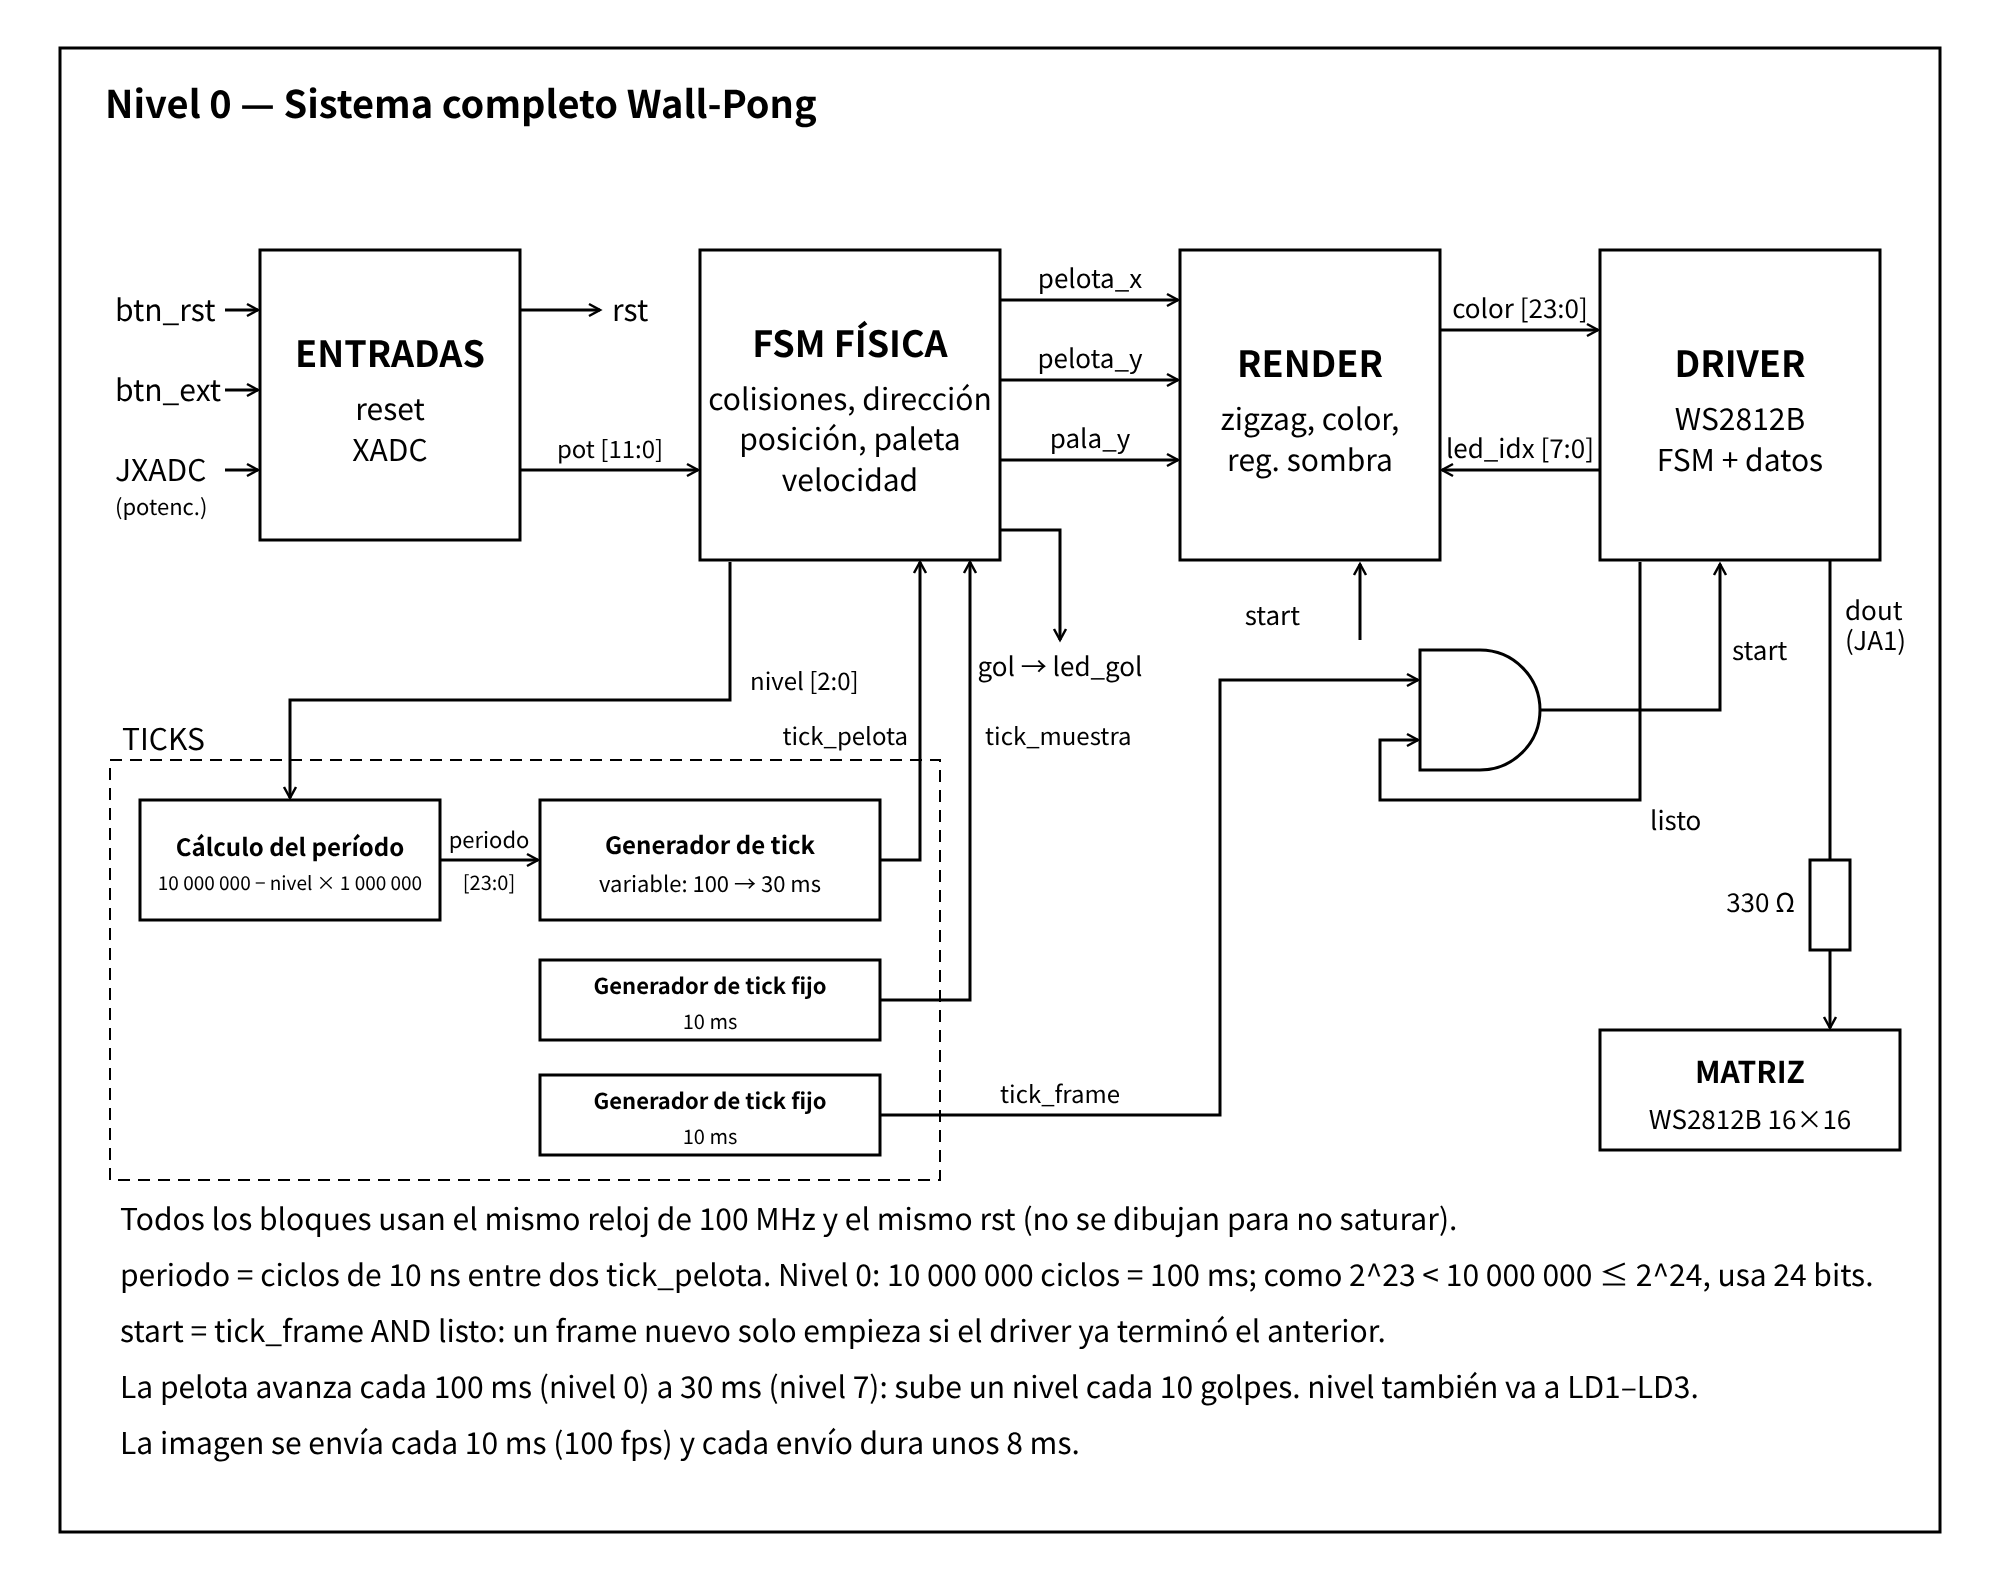
\includegraphics[width=0.82\textwidth]{figuras/00_sistema_completo.png}
\caption{Diagrama de nivel 0. La física avanza con \texttt{tick\_pelota}, cuyo período depende de \texttt{nivel}; el renderizado calcula el color de cada LED al vuelo y el driver lo envía a la matriz.}
\label{fig:sistema}
\end{figure*}

\subsection{Entradas}
El reset (BTNC de la placa OR un botón externo en el Pmod~JB con \emph{pull-down}) pasa por un
sincronizador de dos flip-flops para eliminar la metaestabilidad~\cite{cummings}. El potenciómetro se
conecta a la entrada auxiliar VAUX6 del XADC~\cite{xadc}, configurado en modo de un canal, conversión
continua y promedio de 256 muestras. Al terminar cada conversión (EOC) se lee el registro del canal por
el puerto DRP y, cuando llega DRDY, se guardan los 12 bits útiles \texttt{DO[15:4]}. Como el XADC solo
admite 0--1~V, un divisor de 24~k$\Omega$ con el potenciómetro de 10~k$\Omega$ limita el cursor a
0--0{,}97~V.

\subsection{Ticks y aceleración cada 10 tiros}
Tres contadores generan \texttt{tick\_muestra} y \texttt{tick\_frame} cada 10~ms y \texttt{tick\_pelota}
con período variable:
\begin{equation}
T_{\text{pelota}} = N - \text{nivel}\cdot\frac{N}{10},\quad N = 10^{7}\ \text{ciclos} = 100\ \text{ms},
\end{equation}
es decir 100, 90, \dots, 30~ms para los niveles 0 a 7. El producto por una constante se implementa con
sumas de desplazamientos. El generador compara \texttt{cuenta $\geq$ periodo$-1$} en lugar de usar
igualdad (Fig.~\ref{fig:tickvar}). Si el período baja mientras la cuenta ya superó el nuevo valor, la
igualdad nunca se cumpliría y el contador daría la vuelta completa ($2^{24}$ ciclos
$\approx$ 0{,}17~s con la pelota quieta); con $\geq$ el tick sale en el ciclo siguiente. El período
más grande es $10^{7}$ ciclos y $2^{23} < 10^{7} \le 2^{24}$, por lo que \texttt{periodo} y el contador
usan 24 bits.

El módulo \texttt{control\_velocidad} (Fig.~\ref{fig:velocidad}) tiene un contador de golpes de 4 bits
(0--9) y un registro de nivel de 3 bits. Un golpe es la señal \texttt{choca\_paleta} de la lógica de
colisiones habilitada por \texttt{tick\_pelota}. La habilitación es necesaria porque la condición de
choque se mantiene durante todo el tick y, sin ella, un solo tiro se contaría millones de veces. En el
décimo golpe el contador vuelve a 0 y el nivel sube, saturándose en 7. Un gol o el reset borran ambos
registros, así que cada punto empieza lento. El nivel se muestra en binario en LD1--LD3.

\begin{figure}[t]
\centering
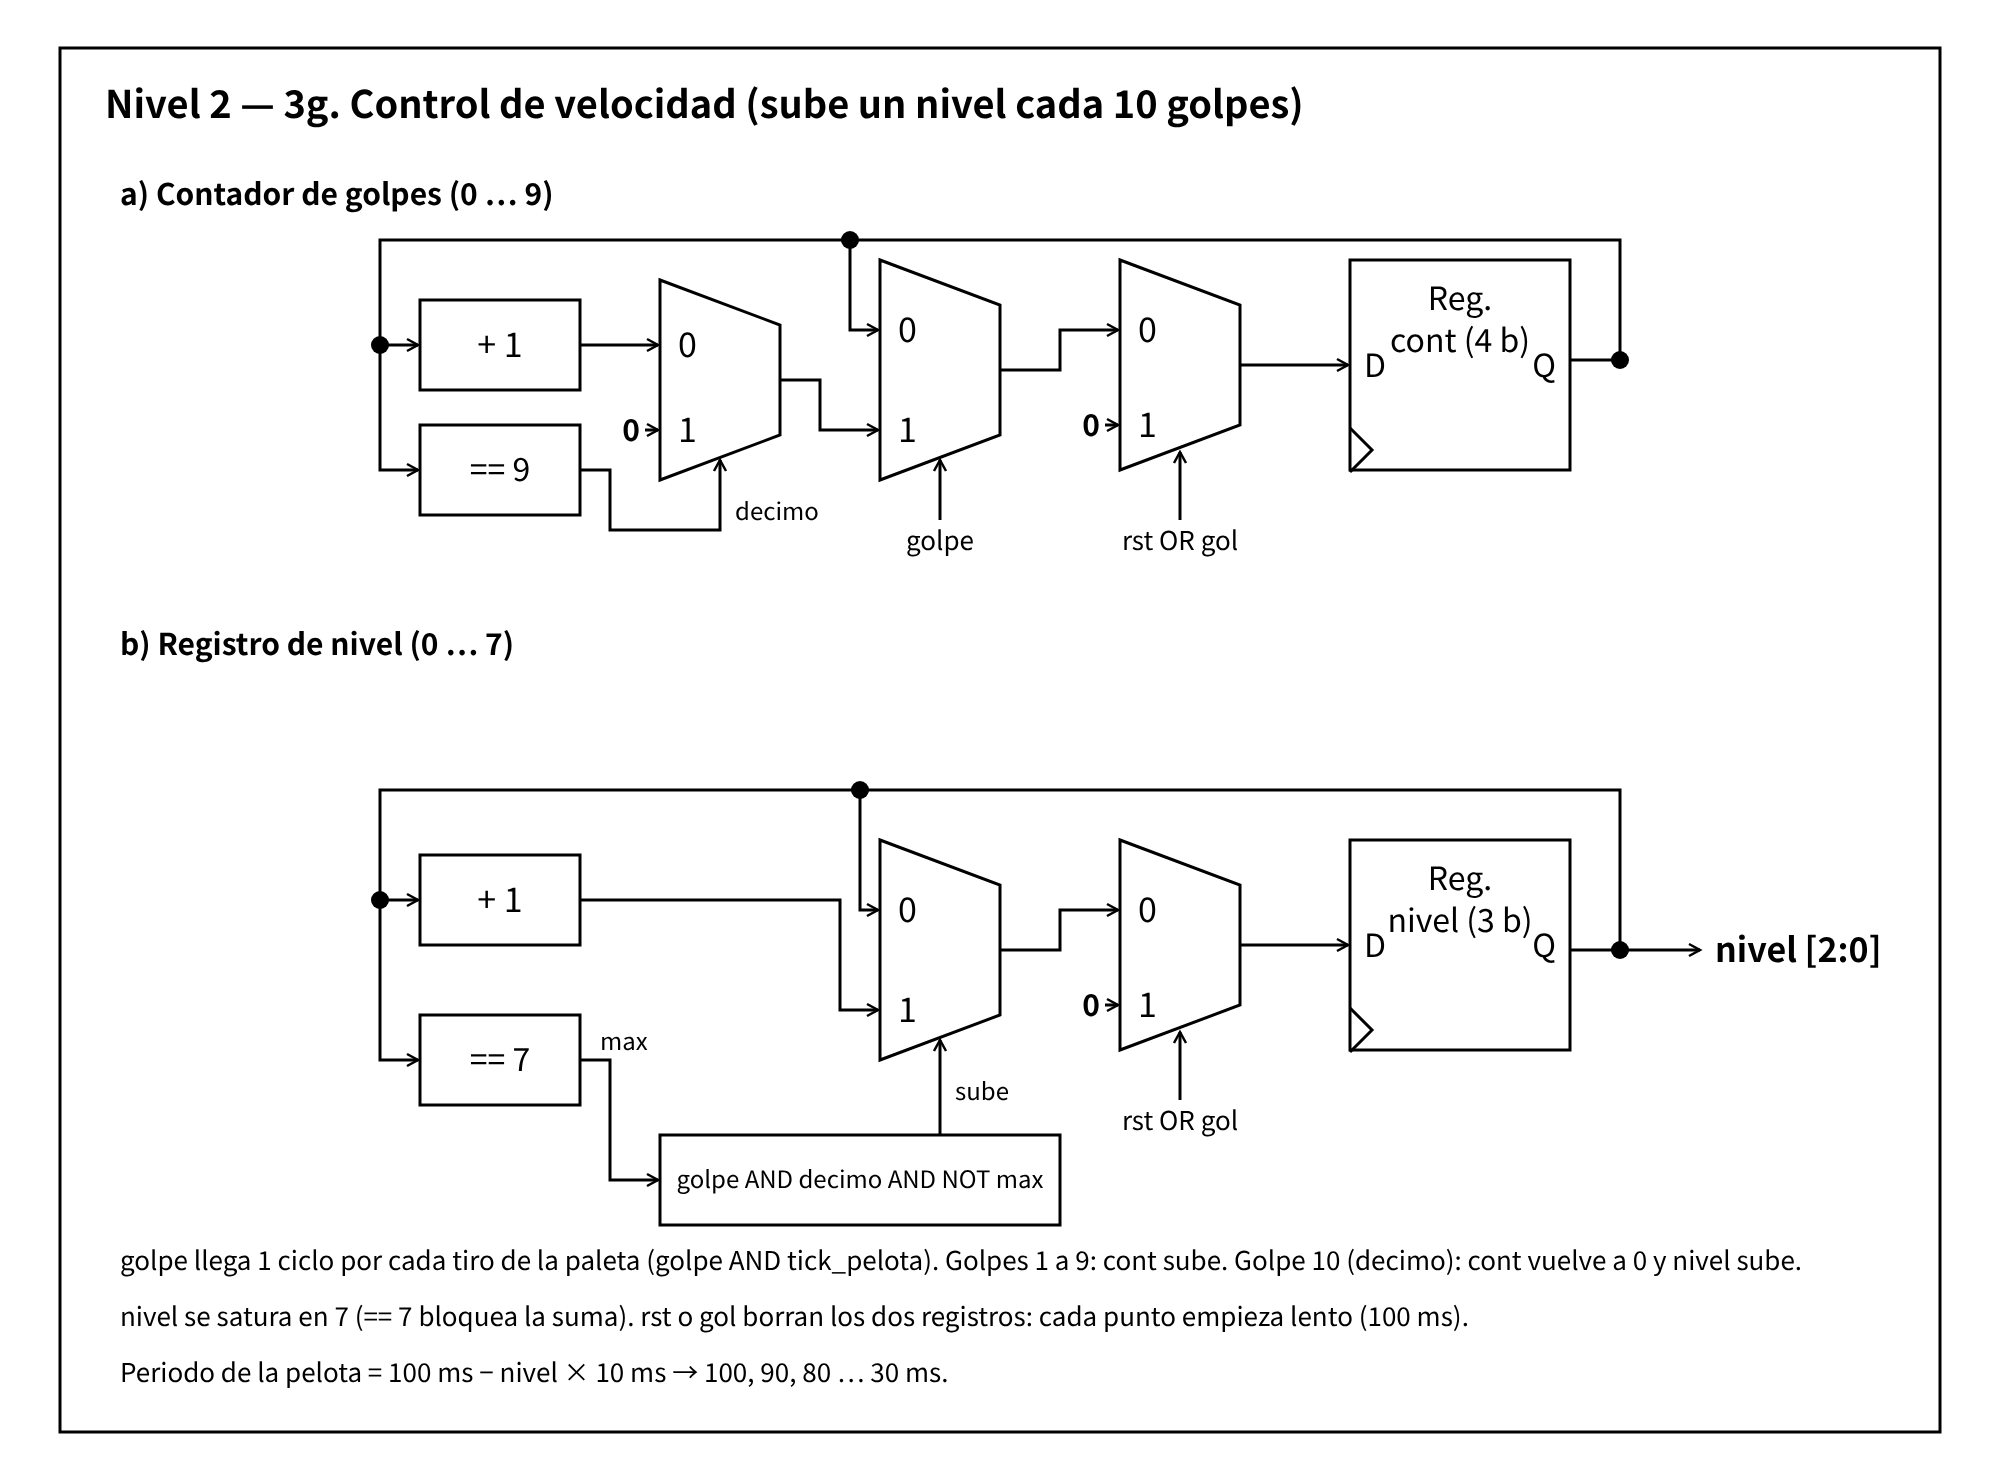
\includegraphics[width=\columnwidth]{figuras/03g_control_velocidad.png}
\caption{Control de velocidad (nivel 2): contador de golpes módulo 10 y registro de nivel saturado en 7, con prioridad de \texttt{rst OR gol}.}
\label{fig:velocidad}
\end{figure}

\subsection{Física del juego}
El estado de la pelota (\texttt{pelota\_x}, \texttt{pelota\_y}, \texttt{dir\_x}, \texttt{dir\_y}) se
guarda en registros con habilitación (Fig.~\ref{fig:fisica}). La lógica combinacional calcula el
siguiente estado: los comparadores detectan techo ($y=0$ subiendo), piso ($y=15$ bajando), pared
($x=14$ hacia la derecha) y paleta ($x=1$ hacia la izquierda con
$\text{pala\_y}\le y\le\text{pala\_y}+2$); una XOR invierte la dirección del eje que choca y un gol
fuerza el saque desde (7,7), de modo que el juego continúa solo después de cada gol.

La paleta se calcula como
$\text{fila} = \lfloor 14\cdot\text{pot}/4096 \rfloor$, implementado como
$\text{pot}\cdot 14 = (\text{pot}\ll4)-(\text{pot}\ll1)$ y tomando los bits altos. Para evitar que la
paleta tiemble cuando el potenciómetro queda entre dos filas, se aplica histéresis: solo se acepta una
fila nueva si el valor está lejos del borde (resto entre 3 y 12 de 16).

\begin{figure}[t]
\centering
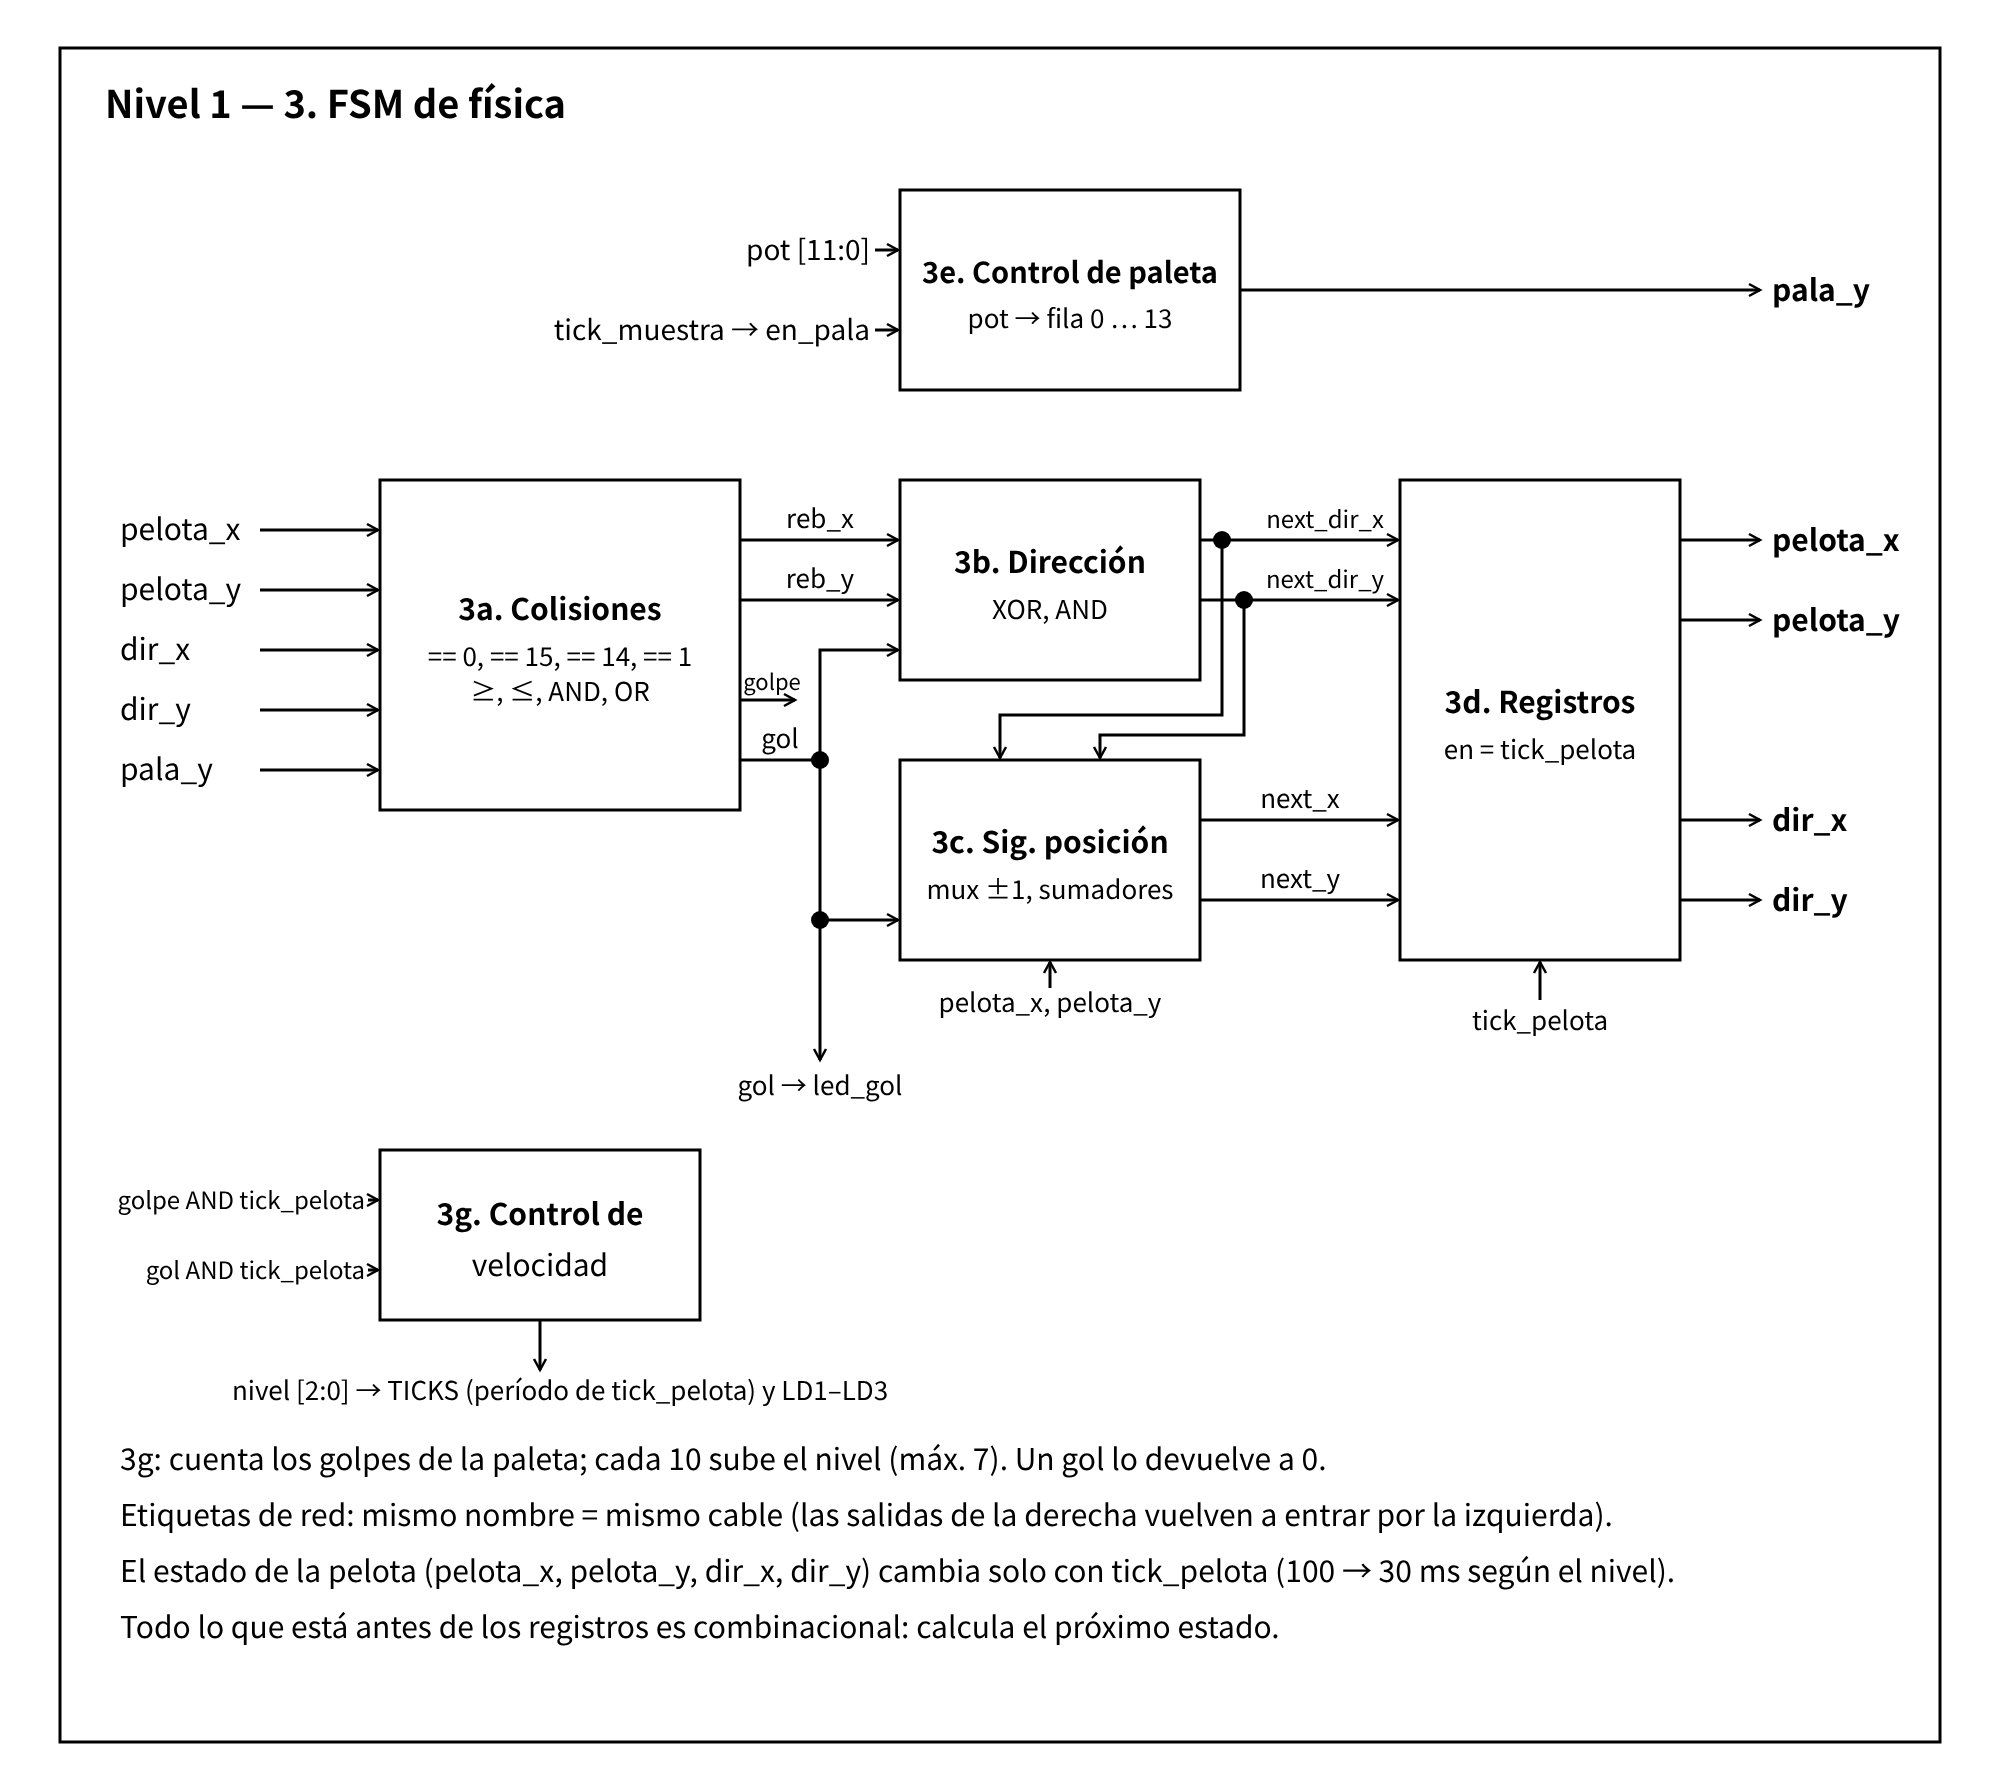
\includegraphics[width=\columnwidth]{figuras/03_fsm_fisica.png}
\caption{FSM de física (nivel 1): lógica combinacional de siguiente estado, registros de la pelota y control de velocidad.}
\label{fig:fisica}
\end{figure}

\subsection{Renderizado sin framebuffer}
En lugar de guardar la imagen en memoria, el color de cada LED se calcula cuando el driver lo pide: el
índice \texttt{led\_idx} (0--255) se convierte en $(x,y)$ con el mapeo en zigzag del panel
($y=\text{idx}[7:4]$, $x=\text{idx}[3:0]\oplus\{4\{y_0\}\}$) y una cadena de multiplexores asigna el color
con prioridad pelota $>$ paleta $>$ pared $>$ fondo. Unos registros sombra copian la posición al inicio
de cada frame para que la imagen no cambie a la mitad del envío.

\subsection{Driver WS2812B}
El WS2812B recibe 24 bits por LED (orden GRB, MSB primero) en un período de 1{,}25~$\mu$s: un 0 está
alto 0{,}35~$\mu$s y un 1, 0{,}70~$\mu$s; un nivel bajo de más de 280~$\mu$s confirma la imagen~\cite{ws2812}.
El driver es una FSM de Moore de cinco estados (IDLE, LOAD\_COLOR, SEND\_BIT, NEXT\_LED, RESET\_LATCH)
más una ruta de datos con un registro de desplazamiento de 24 bits, un contador de período (0--124
ciclos), contadores de bits y de LEDs y un contador de \emph{latch} de 30\,000 ciclos (300~$\mu$s). El
bit se genera comparando el contador de período con 35 o 70 ciclos y la salida \texttt{dout} se
registra para eliminar \emph{glitches}. Un frame nuevo empieza con
\texttt{tick\_frame AND listo}, a 100 imágenes por segundo.

\section{Montaje experimental}
\begin{itemize}
\item \textbf{Hardware:} Digilent Basys~3 (XC7A35T-1CPG236C)~\cite{basys3}; matriz flexible WS2812B
de 16$\times$16 (160$\times$160~mm); potenciómetro lineal B10K con resistencia de 24~k$\Omega$;
botón externo de reset (JB1); fuente de 5~V/3~A con condensador de
1000~$\mu$F y tierra común; resistencia de 330~$\Omega$ en serie con DIN.
\item \textbf{Herramientas:} Icarus Verilog~\cite{iverilog} y GTKWave para simular; AMD Vivado 2026.1 para sintetizar,
implementar y programar~\cite{vivado}; Yosys para estimar recursos.
\item \textbf{Procedimiento:} \texttt{./simular.sh} corre los 23 testbench y resume los resultados; el
script \texttt{vivado/crear\_proyecto.tcl} crea el proyecto, genera el bitstream y los reportes de
utilización y de tiempos. La verificación en la placa se hizo observando la matriz, los LEDs LD0--LD3
y midiendo el voltaje del cursor.
\end{itemize}


\section{Resultados experimentales}

\subsection{Verificación por simulación}
Cada módulo tiene un testbench autoverificable que compara contra el valor esperado e imprime
\texttt{OK}/\texttt{ERROR}. La Tabla~\ref{tab:tb} resume los casos límite principales; en total se
comprueban 138 casos y los 23 testbench pasan. Para confirmar que los testbench detectan errores se
introdujeron fallas a propósito en el diseño (subir de nivel en el golpe 9, comparar con igualdad en el
generador variable) y ambas fueron detectadas.

\begin{table}[t]
\caption{Testbench y casos límite principales}
\label{tab:tb}
\centering
\footnotesize
\begin{tabular}{@{}p{2.2cm}p{5.6cm}@{}}
\toprule
Módulo & Casos verificados \\
\midrule
sincronizador & retardo exacto de 2 ciclos, pulso de 1 ciclo, cambio asíncrono \\
lector\_pot & canal VAUX6, valores 0, 1, 1902 y 4095, \texttt{pot} solo cambia tras DRDY \\
gen.\ tick var. & períodos 10, 7, 2; período reducido con la cuenta ya mayor \\
ticks & los 8 niveles: 100, 90, \dots, 30 ciclos \\
colisiones & 14 casos: bordes, esquinas con doble choque, gol por encima/debajo, \texttt{golpe} \\
control\_paleta & extremos, las 14 filas, histéresis en el borde entre filas \\
control\_velocidad & 9 vs.\ 10 golpes, saturación en 7, gol borra la cuenta, golpe y gol simultáneos \\
fisica\_juego & goles, 2200 ticks con jugador automático: 0 goles y nivel 7 \\
renderizado & zigzag, prioridades en esquinas, cambio a mitad de frame \\
driver & 6144 bits, T0H/T1H de 350/700~ns, latch de 300~$\mu$s \\
wall\_pong\_top & decodifica \texttt{dout}: 256 LEDs correctos por frame, paleta y gol \\
\bottomrule
\end{tabular}
\end{table}

La Fig.~\ref{fig:onda} muestra la simulación de \texttt{control\_velocidad}: el contador recorre 0--9 y
en cada décimo golpe el nivel sube una unidad hasta saturarse en 7; el gol devuelve ambos registros a
cero. En la prueba de integración de la física, el jugador automático devolvió 85 tiros seguidos sin
goles y el nivel coincidió en cada tick con $\min(\lfloor\text{golpes}/10\rfloor, 7)$. El testbench del
driver midió un período de bit de 1250~ns, un nivel bajo de 300{,}6~$\mu$s después del último bit y una
duración de 7{,}69~ms por imagen, menor que el período de 10~ms entre frames.

\begin{figure}[t]
\centering
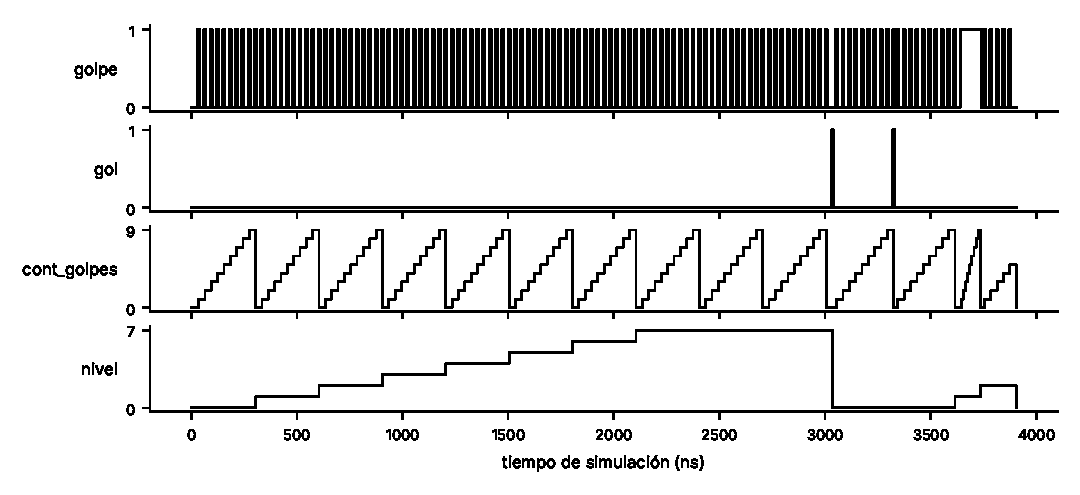
\includegraphics[width=\columnwidth]{figuras/onda_control_velocidad.pdf}
\caption{Simulación de \texttt{control\_velocidad}: el nivel sube cada 10 golpes, se satura en 7 y un gol lo regresa a 0.}
\label{fig:onda}
\end{figure}

\begin{figure}[t]
\centering
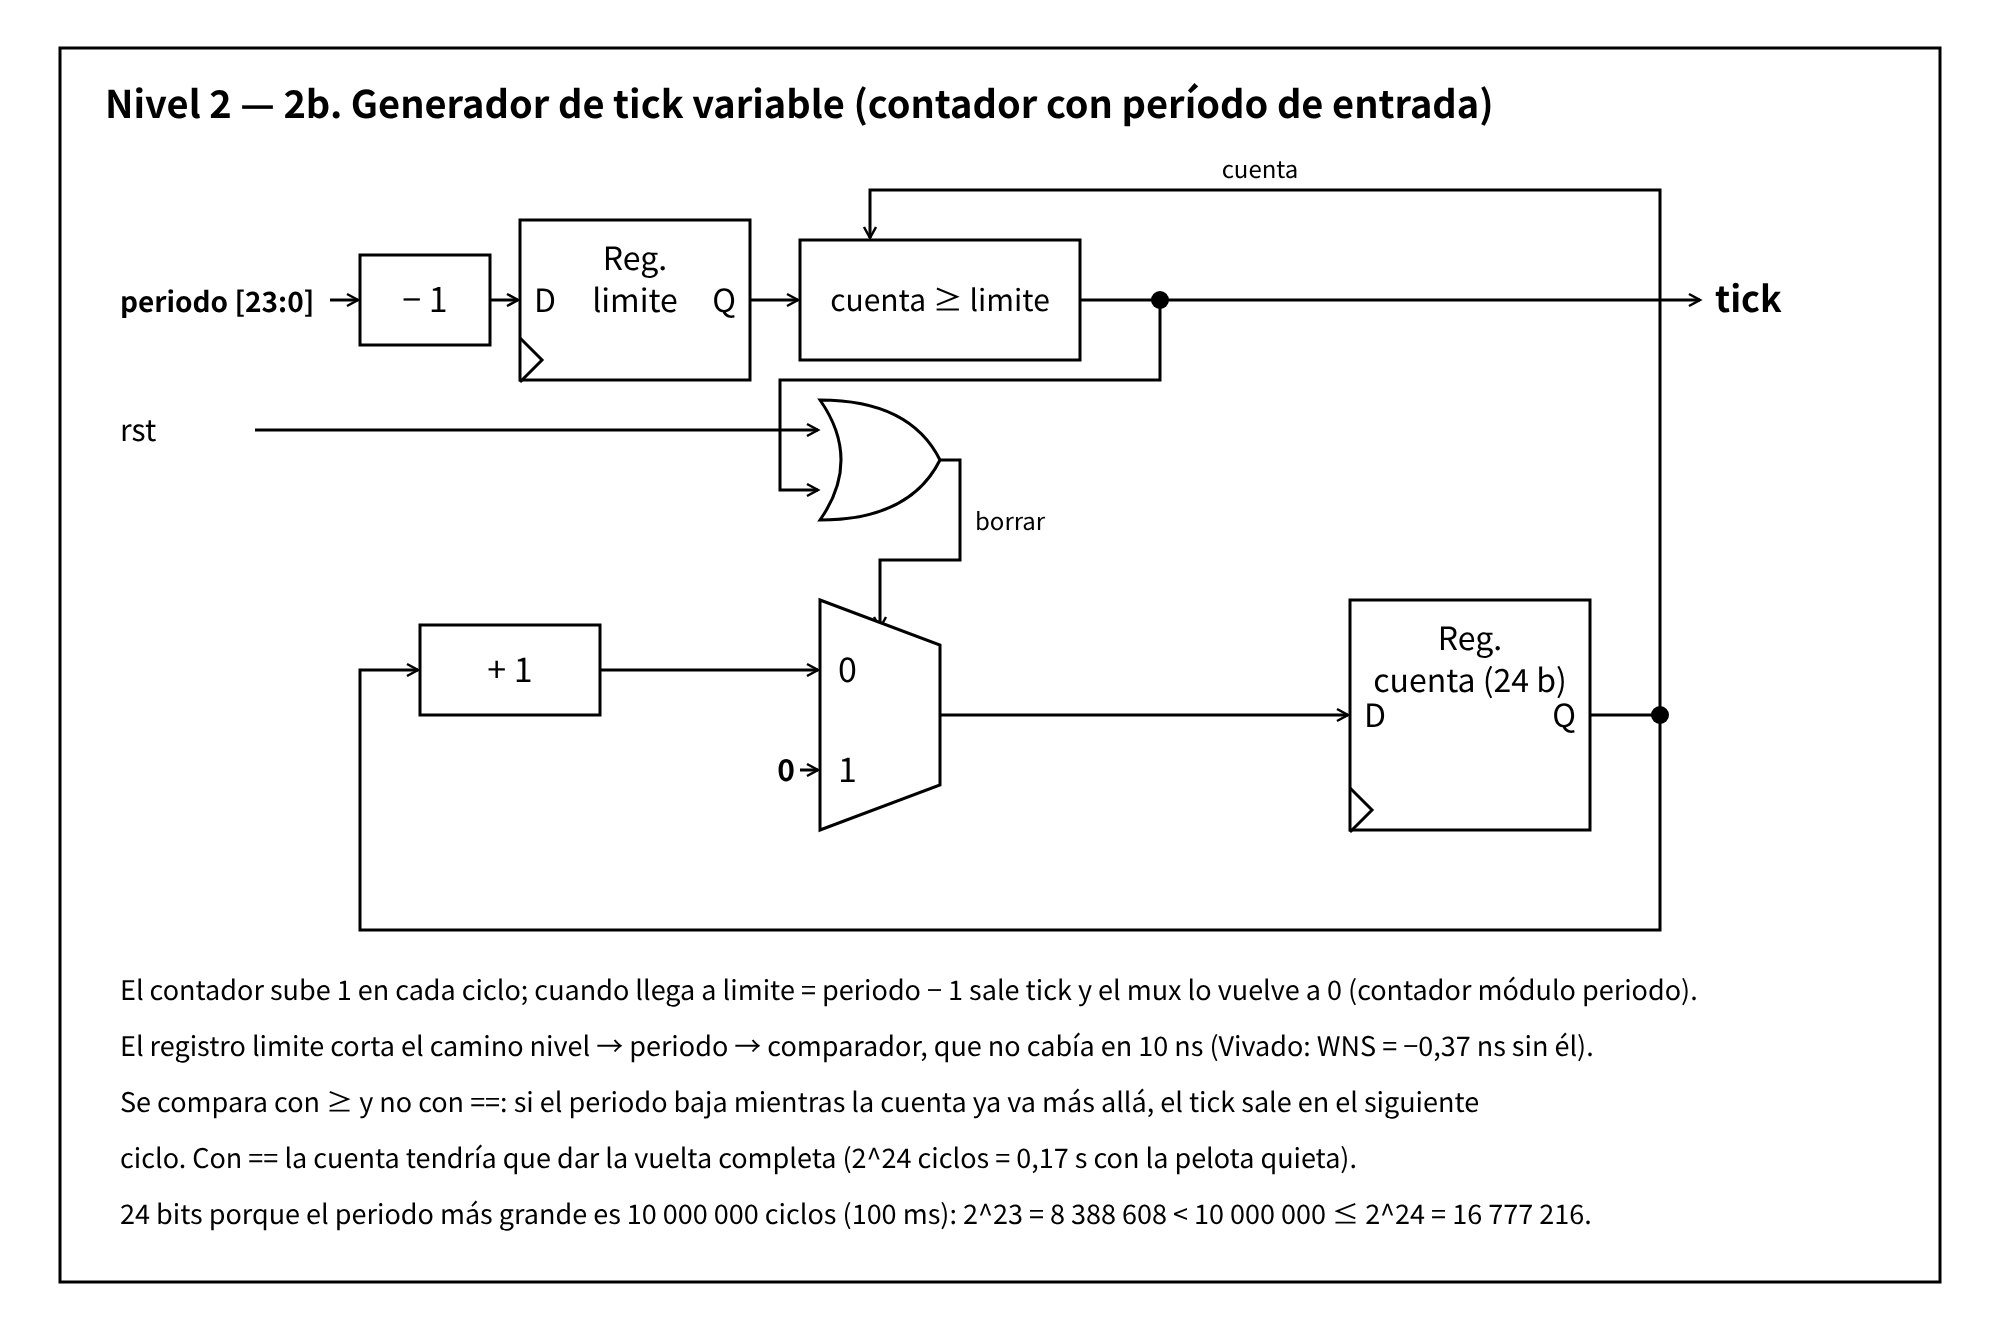
\includegraphics[width=0.92\columnwidth]{figuras/02b_generador_tick_var.png}
\caption{Generador de tick con período variable: el registro \texttt{limite} parte el camino crítico y la comparación con $\geq$ evita que la cuenta dé la vuelta al bajar el período.}
\label{fig:tickvar}
\end{figure}

\subsection{Recursos}
La Tabla~\ref{tab:recursos} muestra los recursos que reporta Vivado después de la implementación, en términos de los elementos del CLB~\cite{clb}. El diseño completo usa menos del 1\,\% del
XC7A35T, gracias a que no hay framebuffer: la imagen se calcula con comparadores en lugar de leerse de
una memoria de 256$\times$24 bits.

\subsection{Tiempos}
La primera implementación no cumplía el reloj de 100~MHz: el peor camino, con 13 niveles de lógica,
iba del registro \texttt{nivel} al contador del generador de tick pasando por el cálculo del período,
la resta $\text{periodo}-1$ y el comparador, con una holgura negativa de $-0{,}367$~ns. Se agregó el
registro \texttt{limite}~$=\text{periodo}-1$ (Fig.~\ref{fig:tickvar}), que parte ese camino en dos; el
costo es que un cambio de nivel se nota 10~ns después, lo que no tiene efecto en el juego. Con ese
cambio la holgura de \emph{setup} quedó en WNS~$=+2{,}613$~ns y la de \emph{hold} en
WHS~$=+0{,}158$~ns, es decir, el diseño funcionaría hasta
$f_{\max}=1/(10-2{,}613)\ \text{ns}\approx 135$~MHz.

\begin{table}[t]
\caption{Recursos usados en la Basys~3 (XC7A35T)}
\label{tab:recursos}
\centering
\footnotesize
\begin{tabular}{@{}lrrr@{}}
\toprule
Recurso & Usados & Disponibles & \% \\
\midrule
LUT & 160 & 20\,800 & 0{,}77 \\
Flip-flops & 170 & 41\,600 & 0{,}41 \\
Slices & 74 & 8\,150 & 0{,}91 \\
XADC & 1 & 1 & 100 \\
BRAM & 0 & 50 & 0 \\
Pines de E/S & 10 & 106 & 9{,}43 \\
\bottomrule
\end{tabular}

\vspace{2pt}
\raggedright\footnotesize Vivado 2026.1, después de la implementación.
\end{table}

\subsection{Pruebas en hardware}
En las pruebas con versiones anteriores del diseño (sin aceleración), la matriz respondió con la señal de
3{,}3~V directa de la FPGA, con 330~$\Omega$ en serie, sin necesidad del buffer 74AHCT125~\cite{ahct}. Al principio la paleta no llegaba a las cuatro filas superiores; la
medición mostró que la entrada negativa XA1\_N estaba al aire y sumaba un desplazamiento de unos
0{,}35~V. Al conectarla a tierra, el cursor recorrió de 0 a 1{,}001~V y la paleta cubrió las 14
posiciones. La aceleración por niveles se verificó en simulación (Sección~IV-A) y en la
implementación cumple los tiempos del reloj de 100~MHz.

\section{Conclusiones}
Se diseñó e implementó un Pong de un jugador en FPGA que cumple el requisito de aumentar la velocidad
cada 10 tiros y agrega una entrada analógica y un display WS2812B con driver propio.
El diseño jerárquico permitió relacionar cada diagrama con un módulo y un testbench, y la verificación
con casos límite encontró problemas reales antes de llegar a la placa. Los más claros son el contador
que da la vuelta si se compara con igualdad y la cuenta repetida de un golpe que dura todo un tick. Usar
un solo reloj con pulsos de habilitación y calcular la imagen al vuelo dio un diseño pequeño (menos del
1\,\% del dispositivo) y fácil de razonar. Como trabajo futuro se propone mostrar el puntaje en la matriz
y agregar el segundo jugador del Pong original.

\section*{Declaración de uso de IA}
Se usó Claude (Anthropic) para consultas técnicas, propuestas de diseño y redacción del código
Verilog, de los testbench, de los scripts y de este documento, a partir de las especificaciones y
decisiones del autor. El detalle por archivo está en \texttt{USO\_DE\_IA.md} del repositorio.

\begin{thebibliography}{9}
\bibitem{ws2812} Worldsemi, ``WS2812B Intelligent control LED integrated light source,'' hoja de datos.
\bibitem{xadc} AMD/Xilinx, ``7 Series FPGAs and Zynq-7000 SoC XADC Dual 12-Bit 1 MSPS Analog-to-Digital Converter User Guide,'' UG480.
\bibitem{basys3} Digilent, ``Basys 3 FPGA Board Reference Manual.''
\bibitem{vivado} AMD/Xilinx, ``Vivado Design Suite User Guide: Synthesis,'' UG901.
\bibitem{clb} AMD/Xilinx, ``7 Series FPGAs Configurable Logic Block User Guide,'' UG474.
\bibitem{cummings} C. E. Cummings, ``Clock Domain Crossing (CDC) Design \& Verification Techniques Using SystemVerilog,'' SNUG, 2008.
\bibitem{harris} D. M. Harris y S. L. Harris, \emph{Digital Design and Computer Architecture}, 2.ª ed. Morgan Kaufmann, 2012.
\bibitem{ahct} Texas Instruments, ``SN74AHCT125 Quadruple Bus Buffer Gates with 3-State Outputs,'' hoja de datos.
\bibitem{iverilog} S. Williams, ``Icarus Verilog,'' \url{https://steveicarus.github.io/iverilog/}.
\end{thebibliography}

\end{document}
